\documentclass{article}
\usepackage[utf8]{inputenc} %кодировка
\usepackage[T2A]{fontenc}
\usepackage[english,russian]{babel} %русификатор 
\usepackage{mathtools} %библиотека матеши
\usepackage[left=1cm,right=1cm,top=2cm,bottom=2cm,bindingoffset=0cm]{geometry} %изменение отступов на листе
\usepackage{amsmath}
\usepackage{graphicx} %библиотека для графики и картинок
\graphicspath{}
\DeclareGraphicsExtensions{.pdf,.png,.jpg}
\usepackage{subcaption}
\usepackage{pgfplots}

\begin{document}


\section{Задачи}
\begin{minipage}{.3\textwidth}
\textbf{Трамвай}\\
$s_0; v_{max} -?$
Найдём зависимоть скорости от расстояния: за dt - $dv=adt$. Так как $dt = \frac{ds}{v}$, то $vdv =(a_0 -bs)ds$. Проинтегрируем и получим: $\int_{0}^{v}vdv = \int_{0}^{s} (a_0 -bs)ds$;
$\frac{v^2}{2} = a_0s -\frac{bs^2}{2}$; $v = \sqrt{(2a_0 -bs)s} $. При $v = 0$; \textbf{$s_0 = \frac{2a_0}{b}$}. $v_{max}$ при $\frac{dv}{ds} = 0$ => $\frac{1}{2}\frac{2a_0-2bs}{\sqrt{2a_0s-bs^2}}=0$. Тогда s = $\frac{a_0}{b} = \frac{s_0}{2}$. Подставим его в v, которое будет max. $v_{max}=\sqrt{2a_0\frac{a_0}{b}-b\frac{a^2_0}{b^2}} = \frac{a_0}{\sqrt{b}}$
\end{minipage}
\hfill
\begin{minipage}{.3\textwidth}
\textbf{Частица y=kx2}\\
$a-?$
Продифференцируем дважды уравнение траектории по времени: $y^.=2kxx^.$; $y^{..} = 2k(x^{.2}+xx^{..})$.
В точке х = 0 величина $|x^.|=v$: $a=(y^{..})_{x=0}=2kv^2$. 
\end{minipage}
\hfill
\begin{minipage}{.3\textwidth}
\textbf{Точка по окружности радиуса r}\\
$a-?$
По усл: $\frac{dv}{dt} = \frac{-v2}{r}$; $dt=\frac{ds}{v}$; $\frac{dv}{v} = \frac{-ds}{r}$. $\int_{v_0}^{v}\frac{dv}{v}=-\int_{0}^{s}\frac{ds}{r}$ => $ln\frac{v}{v_0}=-\frac{s}{r}$ => $v=v_0e^{-\frac{s}{r}}$(s/r).
В данном случае $|a_{\tau}|=a_n$ => $a=\sqrt{2}a_n=\sqrt{2}\frac{v^2}{r} = \sqrt{2}(v_0^2/r)e^{-2s/r}$
\end{minipage}

\section{Задачи}
\begin{minipage}{.3\textwidth}
\textbf{Блок, нерастяжимая нить}\\
$a_1-?$
Выбираем положительное направление оси X вверх, тогда основное уравнение динамики в проеции:
$
\begin{cases}
    m_1a_{1x}=T-m_1g\\
    m_2a_{2x}=T-m_2g
\end{cases}
$. Воспользуемся кинематической связью: $a_1 =a_0+a'$, $a_2=a_0-a'$ ($a'$ - ускорение груза 1 относ блока). Решаем: $m_1(a_0+a')+m_1g=m_2(a_0-a')+m_2g$; $a'=\frac{(m_1-m_2)}{m_1+m_2}(g-a_0)$; $a_1=a_0+a'=\frac{2m_2a_0+(m_1-m_2)g}{m_1+m_2}$
\end{minipage}
\hfill
\begin{minipage}{.3\textwidth}
\textbf{Брусок массы m1}\\
$t_0-?$
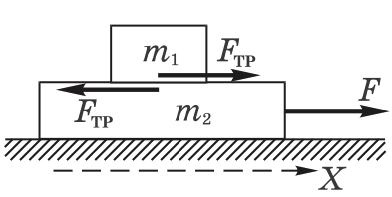
\includegraphics[width=.3\textwidth]{brus.png}
Основное уравнение динамики для бруска будет иметь вид: $m_1a_1=F_{tr}$, $m_2a_2=F-F_{tr}$. При росте F растёт $F_{tr}$ и имеет предел $F_{trmax} = \mu m_1g$ и при его достижении доска начнёт выскальзывать: $a_2\geq a_1$. $(\alpha t -\mu m_1g)/m_2\geq\mu g$(где равенство достиг при $t = t_0$), тогда $t_0=(m_1+m_2)\mu g/\alpha$
\end{minipage}
\hfill
\begin{minipage}{.3\textwidth}
\textbf{Наклонная плоскость}\\
$|a|-?$
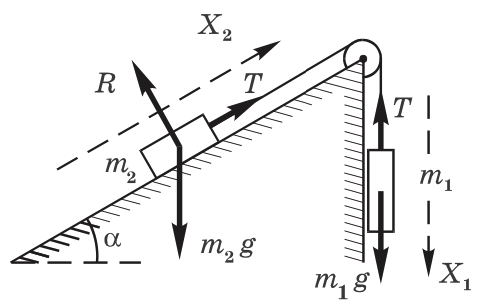
\includegraphics[width=.3\textwidth]{plosk.png}
При отстутствии $F_{tr}$ тело бы начало скользить ввехр по плоскости. При добавлении $F_{tr}$ направление движения не изменится, уменьшится a. Мы сможем определить направление $F_{tr}$ действ на тело $m_2$, когда узнаем направление a при отстутствии $F_{tr}$.
1)$m_1g$, 2)$m_2gsin\alpha= \frac{3}{2}m_1g\frac{1}{2}=\frac{3}{4}m_1g<m_1g$ - тело $m_2$ движется вверх, $F_{tr}$ направлена противоположно. 
$m_1$: $m_1\overline{g}+\overline{T}=m_1\overline{a_1}$; $m_2$: $\overline{T}+m_2\overline{g}+F_{tr}=m_2\overline{a_2}$; $\overline{a_1}|_{x_1}=\overline{a_2}|_{x_2}=a$
$
\begin{cases}
    m_1a=m_1g-T\\
    m_2a=T-m_2gsin\alpha-\mu m_2gcos\alpha
\end{cases}\\; (m_1+m_2)a=m_1g-m_2g(sin\alpha+\mu cos\alpha);
a = \frac{\frac{m_1}{m_2}-(sin\alpha+\mu cos\alpha)}{\frac{m_1}{m_2}+1}\cdot g = 0.05g
$
\end{minipage}

\section{Задачи}
\begin{minipage}{.3\textwidth}
\textbf{Две тележки}\\
$v-?$ Рассмотрим прыжок человека и импульс системы в от прыжка, до преземления невключительно. $(M+m)\overline{v_0}=M\overline{v}+m(\overline{u}+\overline{v})= (M+m)\overline{v}+m\overline{u}$; 
$\overline{v} = \overline{v_0} - \frac{m}{m+M}\overline{u}$; $(\overline{u}+\overline{v})=\overline{v_0}-\frac{m}{m+M}\overline{u}+\overline{u} = \overline{v_0}+\frac{M}{m+M}\overline{u}$;
Далее рассмотрим преземление человека на тележку из состояния полёта: $m(\overline{v_0}+\frac{M}{m+M}\overline{u})+M\overline{v_0}= (m+M)\overline{v'}$; $(m+M)\overline{v_0}+\frac{mM}{m+M}\overline{u}=(m+M)\overline{v'}$; 
$\overline{v'} = \overline{v_0} + \frac{mM}{(m+M)^2}\overline{u}$
\end{minipage}
\hfill
\begin{minipage}{.3\textwidth}
\textbf{два человека}\\
$v-?$ Рассмотрим первый случай, когда один человек спрыгивает с тележки: $(m+M)\overline{v}+m(\overline{u}+\overline{v})$; $\overline{v} = - \frac{m\overline{u}}{M+2m}$
($\overline{v}$ - скорость тележки после прыжка первого человека)
Следующий случай, когда второй человек спрыгивает: $(m+M)(-\frac{m\overline{u}}{M+2m})=M\overline{v'}+m(\overline{u}+\overline{v'}) = (m+M)\overline{v'}+m\overline{u}$
($\overline{v'}$ - скорость тележки после прыжка второго человека).
$(m+M)\overline{v'} = -m\overline{u}(\frac{m+M}{M+2m}+1) = -m\overline{u'}\frac{2M+3m}{(M+2m)}$; $\overline{v'} = - \frac{m\overline{u}(2M+3m)}{(M+2m)(M+m)}$
\end{minipage}
\hfill
\begin{minipage}{.3\textwidth}
\textbf{шайбы*}\\
$T-?$ Рассмотрим ситуацию в ИСО: $T_1=T_2=m_1\frac{v^2_1}{r_1}=m_2\frac{v^2_2}{r_2}=a_{n1}=a_{n2}$.
$r_1+r_2=l$; $r_1m_1=r_2m_2$  |  $r_1=\frac{m_2}{m_1+m_2}l$; $r_2=\frac{m_1}{m_1+m_2}l$
Рассмотрим с-систему: $\overline{P_0}=0$; $m_1v_1=m_2v_2$; $\frac{v_1}{v_2}=\frac{m_2}{m_1}$  |  $v_1=v_c$; $v_c+v_2=v$; $v_1+v_2=v$  |  $v_1=\frac{m_2}{m_1+m_2}v$; $v_2=\frac{m_1}{m_1+m_2}v$  |  $T=\frac{m(\frac{m_2}{m_1+m_2}v)^2}{(\frac{m_2}{m_1+m_2})l} = \frac{m_1m_2}{m_1+m_2}\frac{v^2}{l}$. $R-?$ $R = \frac{v^2_2m_2}{T} = (\frac{m_1+m_2}{m_1})l$
\end{minipage}

\section{Задачи}
\begin{minipage}{.3\textwidth}
\textbf{Космический}\\
$\Delta \alpha-?$ $dm<0$(масса ракеты уменьшается). $(m+dm)(\overline{v}+d\overline{v})-dm(\overline{u}+\overline{v}+d\overline{v})=m\overline{v}$ ($\overline{u}$ - скорость газа относ корабля). После раскрытия скобок: $md\overline{v}-dm\overline{u}=0$.
$d\overline{v}=\frac{dm}{m}\overline{u}\ =>\ dv = v_0d\alpha=-\frac{dm}{m}u$. $v = const = v_0$. $\int_{0}^{\Delta \alpha}d\alpha = -\frac{u}{v_0}\int_{m_0}^{m}\frac{dm}{m}$. 
$\Delta \alpha = \frac{u}{v_0}ln(\frac{m_0}{m})$
\end{minipage}
\hfill
\begin{minipage}{.3\textwidth}
\textbf{Железнодорожная из бункера}\\
$v(t)-?$ $d\overline{p} = \overline{F}dt$. $(m+dm)(\overline{v}+d\overline{v} - m\overline{v} = \overline{F}dt)$. После раскрытия скобок получим: 
$d(m\overline{v}) = \overline{F}dt$. $\Delta m\overline{v} = \overline{F}dt$. При t=0, v(0)=0. $m\overline{v} = \overline{F}t \ ->\ \overline{v} = \frac{\overline{F}t}{m} = \frac{\overline{F}t}{m_0+\mu t} $
\end{minipage}
\hfill
\begin{minipage}{.3\textwidth}
\textbf{Железнодорожная нагружена песком}\\
$v(t)-?$ до: $m,\overline{v}$. после: $(m+dm)(\overline{v}+d\overline{v})$ - тележка. $(-dm)\overline{v}$ - песок в ЛСО.
$d\overline{p} = \overline{F}dt$. $(m+dm)(\overline{v}+d\overline{v})+(-dm)\overline{v} - m\overline{v} = \overline{F}dt$. После раскрытия скобок: 
$md\overline{v} = \overline{F}dt$. $m(t)dv = F dt$. $dv = \frac{F dt}{m(t)} = \frac{F dt}{m_0 -\mu t} = \frac{F}{-\mu}\int_{0}^{t}d(ln(m_0-\mu t))$.
$v(t) = -\frac{F}{\mu}ln(m_0-\mu t)|^{m_0-\mu t}_{m_0}= \frac{F}{\mu}ln(\frac{m_0}{m_0-\mu t})$


\end{minipage}

\section{Задачи}
\begin{minipage}{.3\textwidth}
\textbf{Шарик}\\
$x_{max}-?$ E = const. $T_1+(u_1)_{mg}+(u_1)_{kx} = (u_2)_{mg}+(u_2)_{kx}+T_2$. $T_1=0; (u_1)_{kx} = 0; (u_2)_{mg} = 0; T_2=0$.
$mgx_m = \frac{kx^2_m}{2}$. $x_m = \frac{2mg}{k}$
\end{minipage}
\hfill
\begin{minipage}{.3\textwidth}
\textbf{Небольшое тело}\\
$A_F-?$ $\Delta E = A$. $F=-2m\overline{g}(1-ay)$. $\Delta E = E_2-E_1 = u_2-u_1=mgy=A_F$.
$\delta A_F = (\overline{F}; d\overline{r}) = F_ydy$. $F_y = 2mg(1-ay)$. $\int_{.}^{.}\delta A_F = \int_{0}^{y}2mg(1-ay)dy = 2mgy - mgay^2$. $mgy = 2mg -mgay^2$. $y=\frac{1}{a}$ (весь пусть подъёма s = y-0). $A_F (\frac{1}{2a}) = 2mg\frac{1}{2a} - mga\frac{1}{4a^2} = \frac{mg}{a} - \frac{mg}{4a} = \frac{3}{4} \frac{mg}{2a}$. $\Delta u =mg\frac{1}{2a}=\frac{mg}{2a}$
\end{minipage}
\hfill
\begin{minipage}{.3\textwidth}
\textbf{Три одинаковые}\\
$1)v-?2)A_K - ?$ $\phi = k\frac{q}{a}+k\frac{q}{a}=2k\frac{q}{a}$. В поле конс. Кулоновской силы. $u_1=3k\frac{q^2}{a}$ (потенциальная). $u_1 = \frac{1}{2}\sum_{i!=j}^{}\phi_{ij}q_i = \frac{1}{2}2k\frac{q^2}{a}\cdot3 = 3\frac{kq^2}{a}$.
$E - const$. $E_1=E_2$. '$u_1=u_2+T_2; \ T_1=0$'-> $3k\frac{q^2}{a}= 3k\frac{q^2}{r}+\frac{mv^2}{2}\cdot 3$. $T_2 = \frac{mv^2}{2}+\frac{mv^2}{2}+\frac{mv^2}{2}$. $mv^2=2kq^2(\frac{1}{a}-\frac{1}{r})$. $v = \sqrt{\frac{2kq^2(r-a)}{mra}}$.
$A_K=\frac{u_1}{3} = \frac{kq^2}{a}$
\end{minipage}
\end{document}
